%!TEX root = ../main.tex
%%%%%%%%%%%%%%%%%%%%%%%%%%%%%%%%%%
% Links:
%
% Difficulty:
% Companies: 
%%%%%%%%%%%%%%%%%%%%%%%%%%%%%%%%%%


%\begin{figure}
%	\centering
%	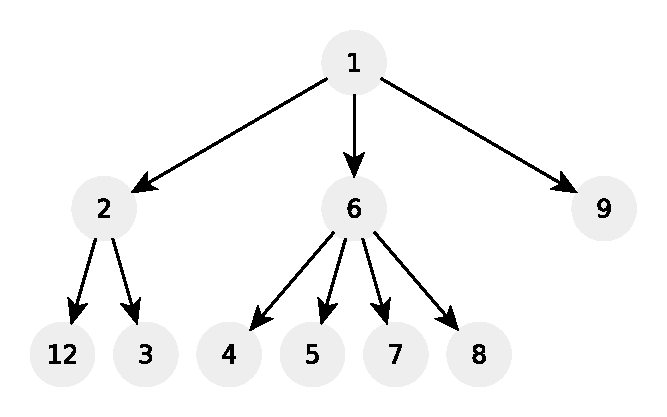
\includegraphics[width=\textwidth]{sources/LRU_cache/images/example1}
%	\caption[Sample short cpation]{Sample Caption}.
%	\label{fig:LRU_cache:example1}
%\end{figure}

\chapter{TITLE OF THE CHAPTER}
\label{ch:LRU_cache}
\section*{Introduction}

\section{Problem statement}
\begin{exercise}
\label{example:LRU_cache:exercice1}

	%example1
	\begin{example}
		\label{example:LRU_cache:example1}
		\hfill \
	}
		
	\end{example}

	%example2
	\begin{example}
		\label{example:LRU_cache:example2}
		\hfill \
		
	\end{example}

	\begin{example}
		\hfill \
	
	\label{ex:LRU_cache:example3}
	\end{example}

	\begin{example}
		\hfill \

	\label{ex:LRU_cache:example4}	
	\end{example}
\end{exercise}

\section{Clarification Questions}

\begin{QandA}
	\item 
	\begin{answered}
		\textit{}
	\end{answered}
	
\end{QandA}

\section{Discussion}
\label{LRU_cache:sec:discussion}


\subsection{Brute-force}
\label{LRU_cache:sec:bruteforce}

\begin{minipage}{\linewidth}
	\lstinputlisting[language=c++, caption={Sample Caption},label=list:LRU_cache]{sources/LRU_cache/LRU_cache_solution1.cpp}
\end{minipage}

